%% Dokumenteinstellungen %%%%%%%%%%%%%%%%%%%%%%%%%%%%%%%%%%%%
\documentclass[a4paper,oneside,10pt,ngerman]{scrartcl}

%% Deutsche Anpassungen %%%%%%%%%%%%%%%%%%%%%%%%%%%%%%%%%%%%%
\usepackage{a4wide}
\usepackage[ngerman]{babel}
\usepackage[T1]{fontenc}
\usepackage[ansinew]{inputenc}
\usepackage{lmodern} %Type1-Schriftart f�r nicht-englische Texte
\usepackage{booktabs}	% sch�nere tabellen

%% Packages f�r Grafiken & Abbildungen %%%%%%%%%%%%%%%%%%%%%%
\usepackage{graphicx} %%Zum Laden von Grafiken
%\usepackage{subfig} %%Teilabbildungen in einer Abbildung
%\usepackage{tikz} %%Vektorgrafiken aus LaTeX heraus erstellen


%% Packages f�r Formeln %%%%%%%%%%%%%%%%%%%%%%%%%%%%%%%%%%%%%
\usepackage{amsmath}
\usepackage{amsthm}
\usepackage{amsfonts}


%% Andere Packages %%%%%%%%%%%%%%%%%%%%%%%%%%%%%%%%%%%%%%%%%%
%\usepackage{a4wide} %%Kleinere Seitenr�nder = mehr Text pro Zeile.
\usepackage{fancyhdr} %%Fancy Kopf- und Fu�zeilen
%\usepackage{longtable} %%F�r Tabellen, die eine Seite �berschreiten
\usepackage{lastpage}
\usepackage[raggedright]{subfigure}
\usepackage[final]{pdfpages}
\includepdfset{pages=-,noautoscale}

%%%%%%%%%%%%%%%%%%%%%%%%%%%%%%%%%%%%%%%%%%%%%%%%%%%%%%%%%%%%%
%% TODO
%%%%%%%%%%%%%%%%%%%%%%%%%%%%%%%%%%%%%%%%%%%%%%%%%%%%%%%%%%%%%
% 
% 
%%%%%%%%%%%%%%%%%%%%%%%%%%%%%%%%%%%%%%%%%%%%%%%%%%%%%%%%%%%%%



%%%%%%%%%%%%%%%%%%%%%%%%%%%%%%%%%%%%%%%%%%%%%%%%%%%%%%%%%%%%%
%% Optionen / Modifikationen
%%%%%%%%%%%%%%%%%%%%%%%%%%%%%%%%%%%%%%%%%%%%%%%%%%%%%%%%%%%%%
%%%%%%%%%%%%%%%%%%%%%%%%%%%%%%%%%%%%%%%%%%%%%%%%%%%%%%%%%%%%%
%%                                                         %%
%%                     EINSTELLUNGEN                       %%
%%                                                         %%
%%%%%%%%%%%%%%%%%%%%%%%%%%%%%%%%%%%%%%%%%%%%%%%%%%%%%%%%%%%%%

%%%%%%%%%%%%%%%%%%%%%%%%%%%%%%%%%%%%%%%%%%%%%%%%%%%%%%%%%%%%%
%% HYPER REF
%%%%%%%%%%%%%%%%%%%%%%%%%%%%%%%%%%%%%%%%%%%%%%%%%%%%%%%%%%%%%
\usepackage[
hyperindex=true,
colorlinks=true,
linkcolor=black,
citecolor=black,
filecolor=black,
menucolor=black,
urlcolor=cyan,
breaklinks=true,
bookmarks=true,
bookmarksopen=false,
bookmarksnumbered=false,
pdfhighlight=/O,
]{hyperref}

%%%%%%%%%%%%%%%%%%%%%%%%%%%%%%%%%%%%%%%%%%%%%%%%%%%%%%%%%%%%%
%% FANCY HEADERS
%%%%%%%%%%%%%%%%%%%%%%%%%%%%%%%%%%%%%%%%%%%%%%%%%%%%%%%%%%%%%
% --- Kopf- und Fusszeilen - {} = rechts (gerade), [] = links (ungerade)
% letzte seite: \pageref{LastPage}
% doppelseitig:
%\lhead{Elektronik: \textbf{Oszilatorschaltungen}}	\chead{}		\rhead{Cyril Stoller und Hannes Stauffer}
%\lfoot{\today}	\cfoot{}		\rfoot{Seite \thepage\ von \pageref{LastPage}}

% einseitig:
%\lhead{\rightmark}			\chead{}					\rhead{}
%\lfoot{\leftmark}			\cfoot{}					\rfoot{Seite \thepage\ von \pageref{\LastPage}}

%\setlength{\headrulewidth}{0.4pt}
%\setlength{\footrulewidth}{0.4pt}


% Formeln r�misch nummerieren
\renewcommand{\theequation}{\Roman{equation}} 

% "Formel" statt "Gleichung"
\def\equationname{Formel}

%%%%%%%%%%%%%%%%%%%%%%%%%%%%%%%%%%%%%%%%%%%%%%%%%%%%%%%%%%%%%
%% DOKUMENT
%%%%%%%%%%%%%%%%%%%%%%%%%%%%%%%%%%%%%%%%%%%%%%%%%%%%%%%%%%%%%
\begin{document}

\title{Praktikum: Gesetz von Stefan-Boltzmann}
\date{\today}
\author{Cyril Stoller}
\maketitle


%%%%%%%%%%%%%%%%%%%%%%%%%%%%%%%%%%%%%%%%%%%%%%%%%%%%%%%%%%%%%
%%                                                         %%
%%         Kapitel / Hauptteil des Dokumentes              %%
%%                                                         %%
%%%%%%%%%%%%%%%%%%%%%%%%%%%%%%%%%%%%%%%%%%%%%%%%%%%%%%%%%%%%%



\section{Ziel}

Dieser Bericht beinhaltet genaue Angaben zur Durchf�hrung und eine Diskussion des \emph{Stefan-Boltzmann} Experiments als Physik-Praktikum in Physik 4. Das Abstrahlungsgesetz von Stefan-Boltzmann soll anhand einer Gl�hbirne verifiziert werden.

\section{Einleitung}
An einer Gl�hbirne soll zuerst die U-I-Kennlinie gemessen werden. Daraus kann der Widerstand berechnet werden. Dieser steigt eigentlich nicht-linear mit der Temperatur des Gl�hwendels an weil Wolfram einen \emph{positiven} Temperaturkoeffizient von $4.8\cdot10^{-3} 1/K$\footnote{dies laut den Praktikumsunterlagen. Laut Wikipedia (\url{http://de.wikipedia.org/wiki/Temperaturkoeffizient}) hat reiner Wolfram einen Temperaturkoeffizien von $4.4\dot10^{-3} 1/K$. Wir vermuten der Gl�hwendeldraht ist noch legiert.} hat.

Aufgrund dieser Messungen kann man dann mit dem Gesetz von Stefan-Boltzmann auf die abgestrahlte Leistung schliessen.

\section{Messung}
Die U-I-Kennlinie wurde mit folgendem Messaufbau nach \autoref{fig:schema}:

\begin{figure}[ht]
	\centering
		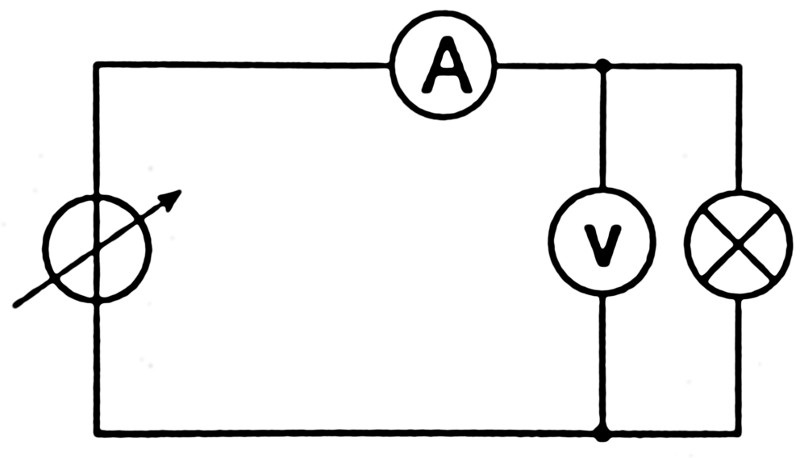
\includegraphics[width=0.30\textwidth]{images/schema.jpg}
	\caption{Messschema}
	\label{fig:schema}
\end{figure}

Die Messwerte sind im Anhang. Herausgekommen der Widerstandsverlauf in \autoref{fig:widerstand}. Der Widerstand wurde berechnet nach $R = U / I$. Man sieht, dass der Widerstand mit steigendem Strom zunimmt. Dies war auch zu erwarten.

\begin{figure}[ht]
	\centering
		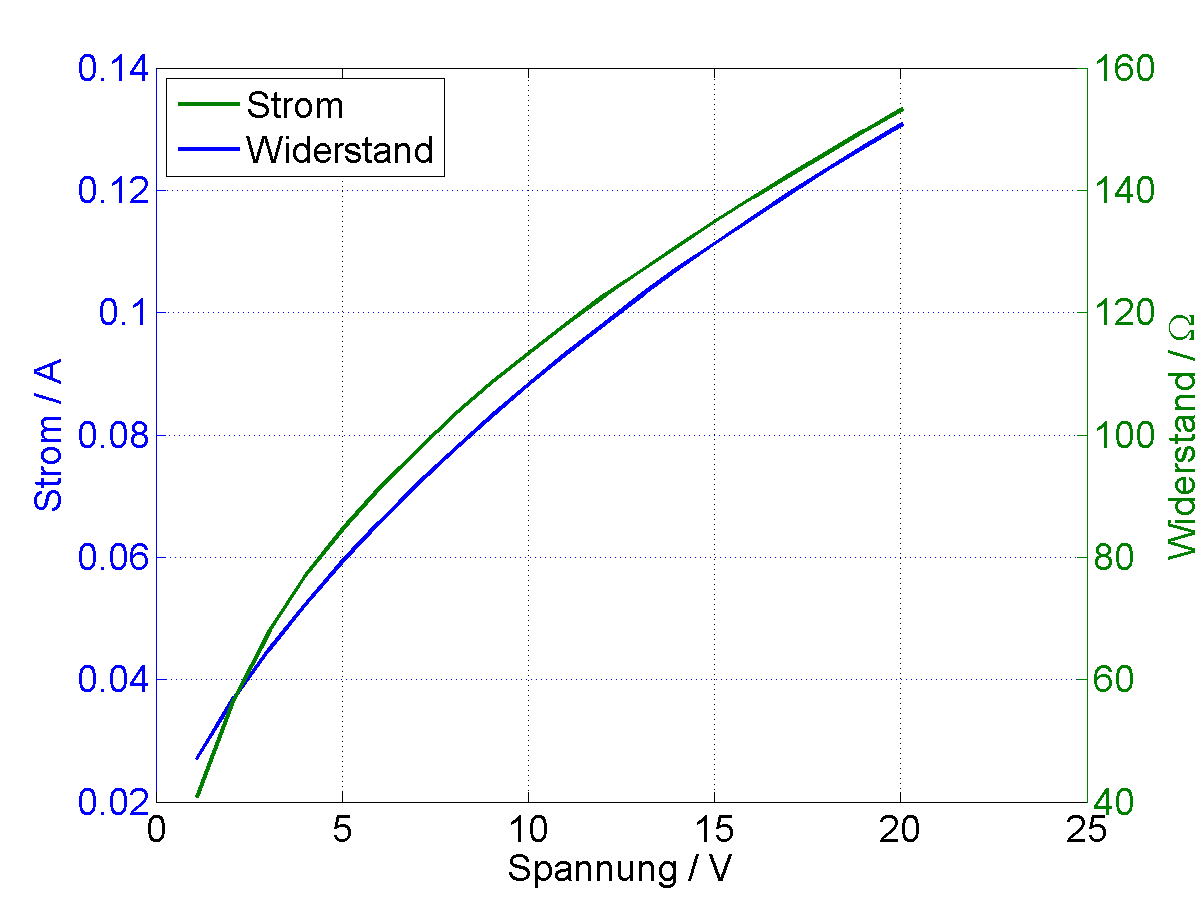
\includegraphics[width=0.70\textwidth]{images/widerstand.png}
	\caption{U-I-Kennlinie mit berechnetem Widerstand}
	\label{fig:widerstand}
\end{figure}

\section{Temperaturberechnung}

Nun wurde die Temperatur berechnet. Die Grundformel daf�r ist die Formel f�r Temperaturwiderst�nde mit linearem Temperaturkoeffizienten\footnote{Aus: \url{http://de.wikipedia.org/wiki/Widerstandsthermometer}}.

\begin{align}
	R_T &= R_{20} (1 + \alpha_{20} (T - T_{umg} )) \\
	T &= \frac{R_T - R_{20}}{R_{20} \cdot \alpha_{20}} + T_{umg}
\end{align}

\begin{align*}
	R_T &: \text{Berechneter Widerstand unter Last} \\
	R_{20} &: \text{Gemessener Widerstand ohne Last} \\
	\alpha_{20} &: \text{Temperaturkoeffizient des Drahtes} \\
	T &: \text{Berechnete Temperatur des Drahtes unter Last}
\end{align*}

\section{Berechnung der Strahlung}

Die abgestrahlte Leistung kann man nun mit folgender Gleichung berechnen:

\begin{align}
	P &= \sigma \cdot \varepsilon \cdot A \cdot (T^4 - T_a^4)
\end{align}

\begin{align*}
	P &: \text{Abstrahlleistung} \\
	\sigma &: \text{Stefan-Boltzmann Konstante} \approx 5.670\cdot10^{-8} \frac{W}{m^2 K^4}\footnotemark \\
	\varepsilon &: \text{Emissiongrad, materialabh�ngig, noch unbekannt} \\
	A &: \text{Oberfl�che, noch unbekannt} \\
	T &: \text{Temperatur}
\end{align*}

\footnotetext{Aus: \url{http://de.wikipedia.org/wiki/Stefan-Boltzmann-Gesetz}}

\section{Vergleich mit gemessener Leistung}

Nun soll der Vorfaktor $k = \sigma \cdot \varepsilon \cdot A$ noch so angepasst werden, dass die gemessene elektrische Leistung ungef�hr mit der berechneten abgestrahlten Leistung �bereinstimmt.

Dies wurde bei $k = 1.5 \cdot 10^{-6} \frac{W}{K^4} \cdot \sigma$ erreicht:

\begin{figure}[ht]
	\centering
		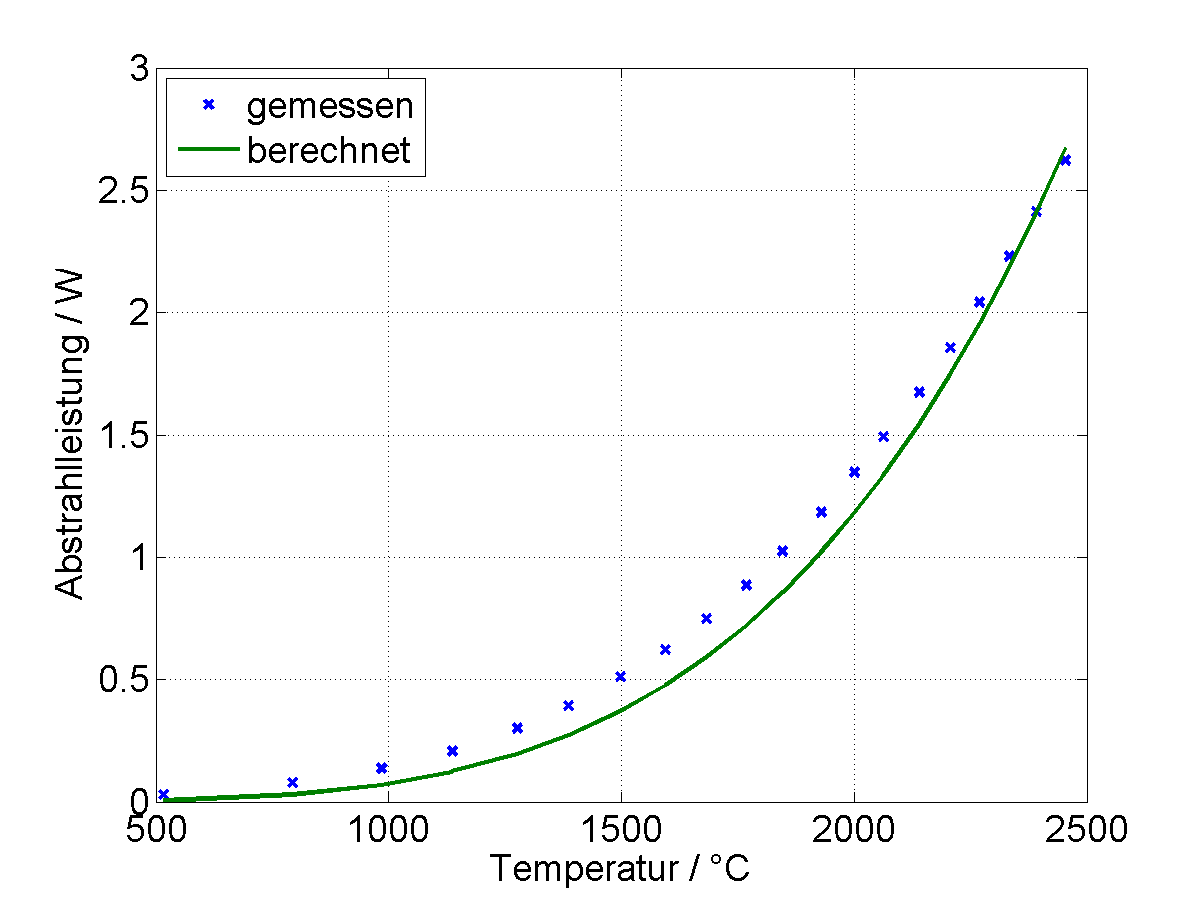
\includegraphics[width=0.70\textwidth]{images/leistung.png}
	\caption{Gemessene und berechnete Leistung}
	\label{fig:leistung}
\end{figure}

Der Koeffizient wurde hier so gew�hlt, dass die Kurve der berechneten Abstrahlleistung leicht \emph{unter} der gemessenen, verbrauchten elektrischen Leistung liegt. Dies aus dem Grund weil neben der Licht-Abstrahlleistung sicher auch noch andere Verlustleistungen auftreten.

\section{Schlussfolgerung}
Die Berechnung der Temperatur k�nnen wir schlecht verifizieren, sie liegt aber im realistischen Bereich.

Nach der Sch�tzung des Parameters $k$ auf die zugrundeliegenden Faktoren $\varepsilon$ und $A$ (weil ja $\sigma$ gegeben ist) zu schliessen, ist schon etwas aufw�ndiger. Im Internet findet man Angaben zum $\varepsilon$ von Wolfram von ca. $0.24$\footnote{\url{https://www.bartec.de/homepage/deu/downloads/produkte/19_temperatur/Ti_Tabelle_Emission_d.pdf}} bei einer Drahttemperatur von $1500$�$C$. In einer anderen Quelle liest man von Drahtdurchmessern im Bereich von $0.02mm$\footnote{\url{http://www.kinder-hd-uni.de/forum1/gluehlampe.html}}.

Also versuchen wir durch berechnen der L�nge des Gl�hdrahtes den gesch�tzten Wert f�r $\varepsilon$ zu testen:

\begin{align*}
	k &= 1.5 \cdot 10^{-6} \frac{W}{K^4} = \sigma \cdot \varepsilon \cdot A \text{ } (\varepsilon = 0.24) \\
	A &= \frac{k}{\sigma \cdot \varepsilon} = 2 \pi r l \text{ (l: L�nge und r: Radius des Drahtes)} \\
	l &= \frac{k}{2 \pi r \cdot \sigma \cdot \varepsilon} = \frac{10^{-6} \frac{W}{K^4} \cdot 5.670\cdot 10^{-8} \frac{W}{m^2 K^4}}{2 \pi \cdot 10 \mu m \cdot 5.670\cdot 10^{-8} \frac{W}{m^2 K^4} \cdot 0.24} = 9.95 cm
\end{align*}

Dies k�nnte gut stimmen, da der Draht eine Spiralform hat.

Der Kurvenverlauf der beiden Leistungen stimmt ebenfalls gut �berein.

\section{Anhang}

Im Anhang ist noch die Messwertetabelle:

\begin{figure}[ht]
		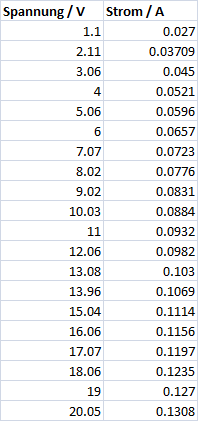
\includegraphics{images/Messwerte.png}
	\label{fig:Messwerte}
\end{figure}


\end{document}
